\chapter{Allgemein}
\label{chap:Allgemein}

\paragraph{Definition Maschinelles Lernen}

\begin{itemize}
    \item Ein System lernt aus Erfahrung E in Hinblick auf eine Klasse von Aufgaben
    T und einem Performanzmaß P wenn seine Leistung bei Aufgaben aus T gemessen mit
    P durch Erfahrungen aus E steigt
    \item z.B T: Schachspielen, P: Prozent der gewonnen Spiele, E: Spiele gegen sich selbst.
\end{itemize}

\paragraph{Was ist Intelligenz?}
\label{par:Was ist Intelligenz?}
\begin{itemize}
    \item Problemlösung, Erinnern, Sprache, Kreativität, Bewusstsein, Überleben
    in komplexen Welten
\end{itemize}

\paragraph{Wissensrepräsentation}
\label{par:Wissensrepraesentation}
\begin{itemize}
    \item Assoziierte Paare (Eingangs und Ausgangsvariablen)
    \item Parameter in algebraischen Ausdrücken
    \item Entscheidungsbäume
    \item Formale Grammatik
    \item Produktionsregel
    \item Formale logikbasierte Ausdrücke
    \item Graphen und Netzwerke
    \item Probabilistische, graphische Modell
    \item Frames, Schemata, Semantische Netze
    \item Prozedurale Kodierung
    \item Taxonomien
    \item Markov Ketten
\end{itemize}

\begin{figure}[!h]
  \centering
  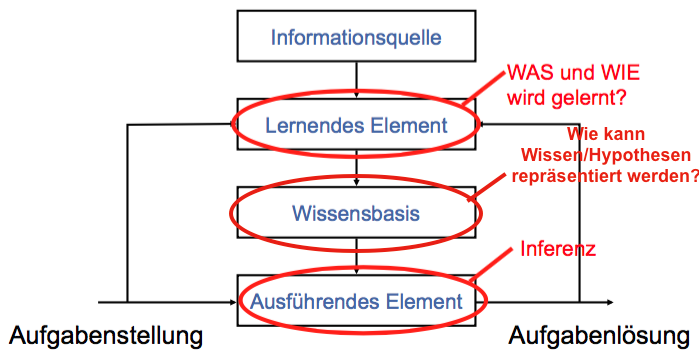
\includegraphics[scale=0.6]{lernendessystem}
  \caption{Komponenten eines Lernenden Systems}
\end{figure}

\paragraph{Inferenz}\mbox{} \\
Vorgang wie ein Programm aus Fakten und Vermutungen (''Korrekte'') Schlüsse
ziehen kann. \\
Aus einer Menge von Formeln A folgt B $\Leftrightarrow$ Es gibt eine Folge von Regeln
um B abzuleiten

\paragraph{Modus Ponens}\mbox{} \\
%$\frac{\text{A, A\rightarrow B}}{\text{B}}$
 Besagt, dass wenn A $\rightarrow$ B und A gilt,
dann gilt auch B. $\frac{A, A \rightarrow B}{B}$

\paragraph{Abduktion} \mbox{} \\
Deduktion beweist, dass etwas ist. Induktion zeigt dass etwas anwendbar ist.
Abduktion zeigt nur, dass etwas sein kann
\begin{enumerate}
    \item alle Menschen sind sterblich
    \item Sokrates ist Mensch
    \item Sokrates ist sterblich
\end{enumerate}
